\chapter{User-level Message Passing}
\label{sec:ump}
Since LMP messaging can be used only for intra-core communication, we need another primitive to support inter-core communication, UMP messaging. We aimed to create a similar interface to LMP for arbitrary-sized messages:

\begin{minted}{c}
errval_t ump_chan_send(struct ump_chan *chan, uint8_t *buf, size_t buflen,
                       struct capref cap);

errval_t ump_chan_recv_blocking(struct ump_chan *chan, uint8_t **buf,
                                size_t *buflen, struct capref *cap);
\end{minted}

\section{Ringbuffers}
The fundamental building block of our user-level message passing is a ring-buffer data structure. The ring-buffer is somewhat unique however, the implementation is optimised by reserving an entire cache line for data transfer. The ring-buffers work by mapping in a shared region of memory between the two communicating processes. One limitation of this method is that they are single writer/single reader data structures. The data structure itself was fairly trivial to implement as we were able to use an array, in the case we reached the end of the array, we would simply just jump back to the start of the array. The cache line is split into two segments, one data segment and another status segment, obviously the status segment is quite small at just a single word, while data data segment takes up the rest of the cache line. The image below displays the state of a ring-buffer at some point of execution.

\begin{figure}[ht]
	    \centering
	        \scalebox{0.5} {
	            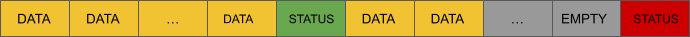
\includegraphics{figs/ringbuffer.png}
	        }
	    \caption{Ringbuffer}
	    \label{fig:ringbuffer}
	\end{figure}

\subsection{Writer}
The ring-buffer operates in two different modes, one is a `write' mode where the ring-buffer is used to relay information to another domain. In this mode of operation, writes occur by simply waiting for the status segment to be \mintinline{c}{BUFFER_WAITING}, this value indicates that the other domain is now waiting for input and therefore we can now write to the associated data segment of that specific cache line. For example, if we refer to figure \ref{fig:ringbuffer} we can see the writer in the process of filing up the data slots for the second cache line, after this has happened the status segment of the second cache line will be set to \mintinline{c}{BUFFER_READY} and therefore will be available for the reading domain to read from. 

\subsection{Reader}
As mentioned previously, the ring-buffer operates in two different modes, the `read' mode is how a domain is able to receive a message from another domain. Here, we simply wait till our status segment is set to \mintinline{c}{BUFFER_READY}, this value indicates that the writing domain has a cache line worth of information ready to be consumed by the reading domain. In this case, we read these values into a buffer and update the status segment to \mintinline{c}{BUFFER_WAITING}, which will allow the writer to reuse this memory again. 

\subsection{Memory Consistency}
One problem with how the ring-buffers work on ARM processors is that the ARM processors implement quite a weak form of memory consistency, in order to address this issue we had to add barriers before reading the status segments and barriers again before updating status registers. The barriers before the reading helped ensure that all memory was up to date and the barrier before updating ensured that all the read/write operations had propagated before the status was set.  

\section{UMP channel}
Our ringbuffer is a single writer, single reader data structure. Therefore, in order to support a two-way communication we employed two ringbuffers, one for each direction. We split a frame shared between the two communicating ends into two halves as shown on Figure \ref{fig:ump_panes}. Each half contains a ringbuffer. The first endpoint is a sender for one ringbuffer and a receiver for the other. The second endpoint, unsurprisingly, receives where the first sends and sends where the first receives.

\begin{figure}[ht]
    \centering
        \scalebox{0.8}{
            \includesvg{./figs/ump_panes.svg}
        }
    \caption{Using two ringbuffers to build a two-way UMP channel.}
    \label{fig:ump_panes}
\end{figure}

Alternatively, it would be possible to use a more sophisticated ringbuffer supporting multiple writers and readers. However, we found the approach with two ringbuffers much simpler.

In the initial implementation, the receiver explicitly polled the corresponding ringbuffer in a separate thread. For convenience, we later incorporated our UMP channel into \mintinline{c}{waitset} so that we could build an abstraction over UMP and LMP channels. Finally, to give 

\section{Sending capabilities and big messages}
To send messages of arbitrary sizes we use an encoding very similar to the one we used for LMP which just contains the buffer length in the header. To support sending frame capabilities between two  \mintinline{c}{init} domains, we also include enough information to forge the frame capability in the foreign \mintinline{c}{init}. Each UMP message is $56$ bytes long and we use the first message just for the header. Here's how it looks:

\begin{figure}[ht]
    \centering
        \scalebox{0.8}{
            \includesvg{./figs/ump_message.svg}
        }
    \caption{A general format of a message on a UMP channel.}
    \label{fig:ump_msg}
\end{figure}

The \mintinline{c}{frame.base}, \mintinline{c}{frame.bytes}, and \mintinline{c}{core_id} are used to forge a frame capability on the receiving end.

Also note that the full 56B are used for the header -- there's definitely room for an optimization. however as seen on the figure \ref{fig:ump_rtt} the RTT grows linearly with the message size (it's a log plot) so saving a single UMP message does not make a big difference. Therefore, we chose to keep things simple.

\subsection{Benchmarks}
\label{sec:ump_bench}

The Figure \ref{fig:ump_rtt} shows RTT scaling of our implementation of messages over UMP. First, it's important to notice that for small messages the difference to LMP is small (16B over LMP takes 26$\mu$s and over UMP 17$\mu$s\footnote{These numbers should be taken with a grain of salt because we just took an average of many runs so we don't know how the distribution looks.}). However, for big messages, UMP scales much better. We attribute this to the fact that since the communication is cross-core, the reader and writer can process data in parallel and no context switches are needed as opposed to the LMP.


\begin{figure}[ht]
    \centering
        \scalebox{0.8}{
            \includesvg{./figs/ump_really_big.svg}
        }
    \caption{Graph showing RTT of a single message over UMP across cores.}
    \label{fig:ump_rtt}
\end{figure}

\begin{hindsight}
Similarly to the implementation of arbitrary-sized messaged over LMP, we ended up quite satisfied with our UMP channels. But again, they didn't get to be fully appreciated because the RPC layer was our bottleneck by far. It would definitely be interesting to add a new "non-greedy" version of the UMP channels facilitating IPIs to see how big would be the performance hit.
\end{hindsight}

\section{All-to-all init UMP channels}
To avoid routing all communication through a single core, we added a UMP channel between each \mintinline{c}{init} domain in both directions (since our RPCs have a client-server structure). This means 12 UMP channels in total.

We achieve this by allocating a big enough frame on core 0 and passing this frame to each core's \mintinline{c}{init} through the \mintinline{c}{struct armv8_core_data}. The memory of each channel is predefined so each core knows how to initialize their channels.

It is of a bit hazardous as every ini\mintinline{c}{init} has access to every init-to-init UMP channel. There are of course safer approaches with better encapsulation, but we went for this implementation because of its simplicity. The channels turned out to be very useful, mostly for the Nameservice.

\section{A full binding system for arbitrary process-to-process communication}
\label{sec:full_binding_ump}

The code for this was deprecated and deleted since it was replaced by the name services.
We were providing the following interface:

\begin{minted}{c}
errval_t aos_rpc_create_server_on_port(struct aos_rpc_server_socket *server,
                                       uint16_t port);
errval_t aos_rpc_accept_connection(struct aos_rpc_server_socket *server,
                                   struct aos_rpc_client *socket);
errval_t aos_rpc_connect_to_port(struct aos_rpc_client *client,
                                uint16_t port);
\end{minted}

This allowed to any user process to create a server on a port. The port mapping was handled by a shared memory regions between all init processes on each core. This made it possible that a port can be acquired by using \mintinline{c}{atomic_cmpset_int()} and no other process was able to get the same port. Inside the port map the init would write its core s.t. other client that want to connect can contact the init on the right core to establish the connection. \mintinline{c}{aos_rpc_create_server_on_port()} created a LMP channel to the init on the same core that also acquired the port for us. \mintinline{c}{aos_rpc_accept_connection()} wait blockingly on that LMP channel waiting init to inform us about a client being connected.  \mintinline{c}{aos_rpc_connect_to_port()} will create a UMP frame send it to our init, which will forward the request to the owning core (by a lookup in the port map). The init on the owning core will then find the LMP channel for this port and send the UMP frame to the server waiting for it, this will unblock \mintinline{c}{aos_rpc_accept_connection} and return a connection to the other process.

(The commit hash of this was "43404b87930af75be8b2e0067d8e22b7fdc76d3d")
%nice